\documentclass[10pt,letterpaper]{article}
\usepackage[utf8x]{inputenc}
\usepackage{ucs}
\usepackage[spanish]{babel}
\usepackage{amsmath}
\usepackage{amsfonts}
\usepackage{amssymb}
\usepackage{graphicx}
\sloppy
\setlength{\parindent}{0pt}
\usepackage[none]{hyphenat}
\usepackage[left=0.5cm,right=0.5cm,top=0.5cm,bottom=0.5cm]{geometry}
\author{F\'elix Ernesto Charry Pastrana}
\begin{document}
\textbf{Universidad Nacional Autónoma de México}\\
Presentado a: \textbf{Santiago Caballero}\\ 
Presentado por: \textbf{F. E. Charry-Pastrana}\\
Maestría en Ciencias Físicas \\
Introducción a la física computacional \\
3 de mayo de 2018 \\
\begin{center}
\textbf{\begin{LARGE}
Shooting method: simple pendulum
\end{LARGE}}
\end{center}
Las ecuaciones para el péndulo simple son: 
\begin{eqnarray}
\dot{p} &=& - \sin(\theta ),\\
\dot{\theta} &=& p,
\end{eqnarray}
con $m=1$, $g=1$, $l=1$ y la energía constante como $E = \dfrac{p^2}{2} + 1 - \cos(\theta)$.\\ \\
El método de ``shooting'' se utilizó para encontrar aquellas soluciones para las cuales el ángulo inicial, $\theta_0$, fuese $\theta_0 = \dfrac{\pi}{2}$ y el ángulo para $t=10$ fuese el mismo ángulo inicial, $\theta(t=10) = \theta_0$.
\\ \\
\section{Solución encontrada en clase}
La solución que se encontró en clase, utilizando como \textit{semilla} para $p_0 = 1$, se muestra en la Figura \ref{Fig-Clase}.
\begin{figure}[h]
\centering
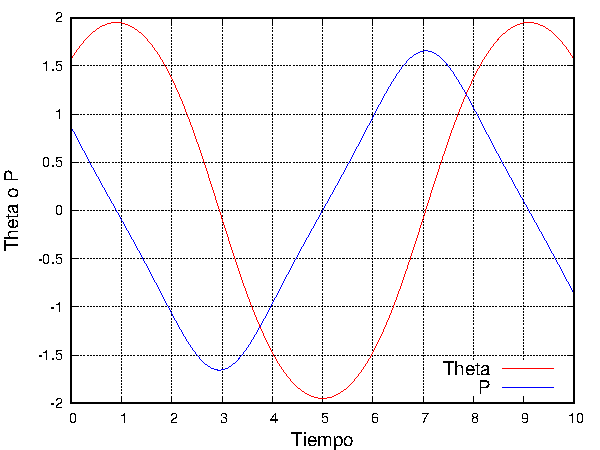
\includegraphics[scale=1]{Solucion.pdf}
\caption{Solución encontrada en clase para $\theta$ y $p$ en función del tiempo, $t$, utilizando como semilla para $p_0 = 1$. }\label{Fig-Clase}
\end{figure}
\section{Soluciones en función de la semilla $p_0$}
El valor inicial para una solución que cumplan las condiciones del problema, $\theta_0 = \theta(t=10) = \dfrac{\pi}{2}$, dependen del valor de la semilla para el momento inicial. En la Figura \ref{Fig-Semilla} se muestra esta dependencia y se observa que, en el rango de $p_{\text{semilla}} = [-\pi, \pi]$, existen \textbf{tres} valores aceptables para $p_0 = \{-1.24,\, 0.86, \,1.24\}$. Aunque se reporta solución para $p_0 = -1.41$, esta ``solución'' se cree que se debe a un error numérico referente al número de iteraciones.
\begin{figure}
\centering
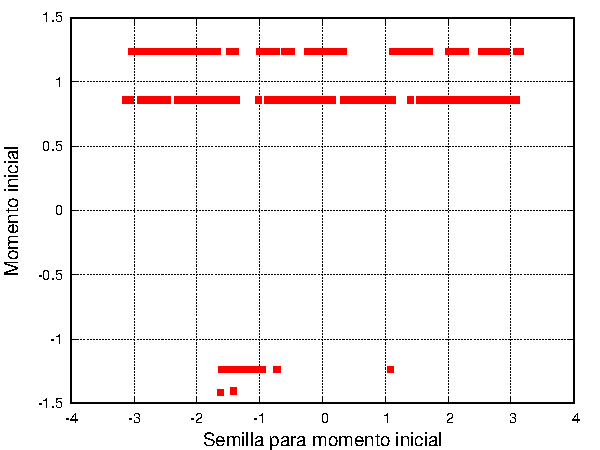
\includegraphics[scale=1]{Grafica_P0.pdf}
\caption{Dependencia del valor inicial de $p_0$ en función de la semilla.}\label{Fig-Semilla}
\end{figure}
\section{Soluciones}
En la Figura \ref{Fig-Sol} se muestra las soluciones aceptables. \\ \\
$p_0 = 0.86$ presenta una energía de $E = 1.34$. \\
$p_0 = -1.24$ y $p_0 = 1.24$ presentan una degeneración en la energía, ambos con $E = 1.76$. \\
$p_0 = -1.41$ no es una solución aceptable.
\begin{figure}
\centering
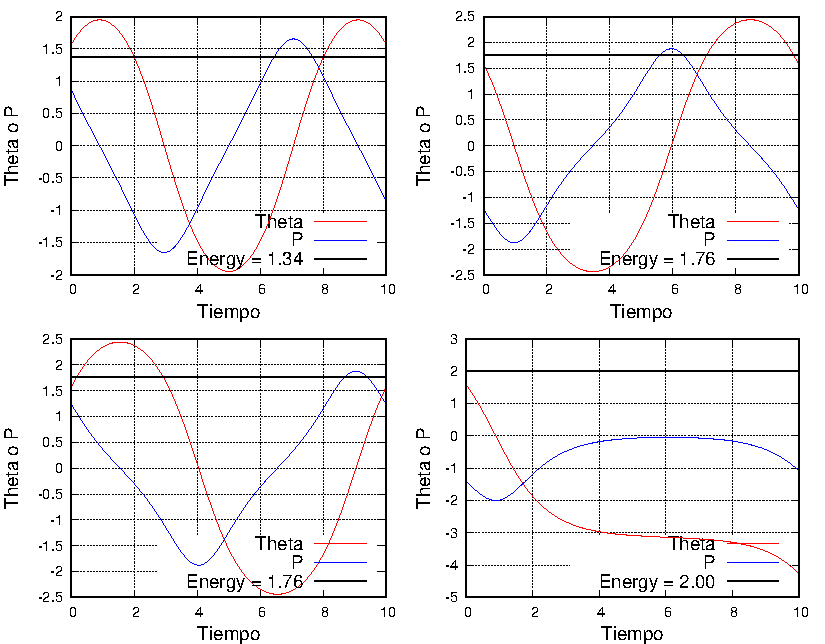
\includegraphics[scale=1.5]{Grafica.pdf}
\caption{Soluciones de $\theta$, $p$ y energía en función del tiempo que cumplen con $\theta_0 = \theta(t=10) = \dfrac{\pi}{2}$. Se muestra ``solución'' para $p_0 = -1.41$.}\label{Fig-Sol}
\end{figure}
\end{document}